\documentclass[tikz]{standalone}

\usepackage[latin1]{inputenc}
\usepackage{tikz}

% GNUPL
\begin{document}
\pagestyle{empty}


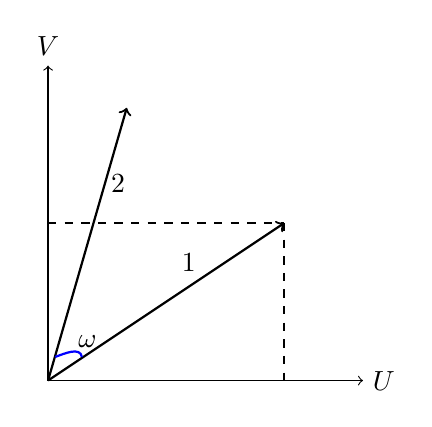
\begin{tikzpicture}
    %\draw[very thin,color=gray] (-1,1.1) grid (3.9,3.9);
    \draw[->] (0,0) -- (4,0) node[right] {$U$};
    \draw[->] (0,0) -- (0,4) node[above] {$V$};
    \draw [black, dashed, semithick] (0,2) -- (3,2);
    \draw [black, dashed, semithick] (3,2) -- (3,0);
    \draw [black, thick] [->] (0,0) -- (3,2);
    \draw [black, thick] [->] (0,0) -- (1,3.4641);
    \draw[blue,thick] (0.091,0.3) to [out=20,in=100] (0.43,0.3);
    \coordinate [label=left:$1$] (3) at (2,1.5);
    \coordinate [label=left:$2$] (4) at (1.1,2.5);
    \coordinate [label=center:$\omega$] (1) at (0.5,0.5);
    
\end{tikzpicture}


\end{document}